% Options for packages loaded elsewhere
\PassOptionsToPackage{unicode}{hyperref}
\PassOptionsToPackage{hyphens}{url}
\PassOptionsToPackage{dvipsnames,svgnames,x11names}{xcolor}
%
\documentclass[
  letterpaper,
  DIV=11,
  numbers=noendperiod]{scrartcl}

\usepackage{amsmath,amssymb}
\usepackage{iftex}
\ifPDFTeX
  \usepackage[T1]{fontenc}
  \usepackage[utf8]{inputenc}
  \usepackage{textcomp} % provide euro and other symbols
\else % if luatex or xetex
  \usepackage{unicode-math}
  \defaultfontfeatures{Scale=MatchLowercase}
  \defaultfontfeatures[\rmfamily]{Ligatures=TeX,Scale=1}
\fi
\usepackage{lmodern}
\ifPDFTeX\else  
    % xetex/luatex font selection
\fi
% Use upquote if available, for straight quotes in verbatim environments
\IfFileExists{upquote.sty}{\usepackage{upquote}}{}
\IfFileExists{microtype.sty}{% use microtype if available
  \usepackage[]{microtype}
  \UseMicrotypeSet[protrusion]{basicmath} % disable protrusion for tt fonts
}{}
\makeatletter
\@ifundefined{KOMAClassName}{% if non-KOMA class
  \IfFileExists{parskip.sty}{%
    \usepackage{parskip}
  }{% else
    \setlength{\parindent}{0pt}
    \setlength{\parskip}{6pt plus 2pt minus 1pt}}
}{% if KOMA class
  \KOMAoptions{parskip=half}}
\makeatother
\usepackage{xcolor}
\setlength{\emergencystretch}{3em} % prevent overfull lines
\setcounter{secnumdepth}{5}
% Make \paragraph and \subparagraph free-standing
\ifx\paragraph\undefined\else
  \let\oldparagraph\paragraph
  \renewcommand{\paragraph}[1]{\oldparagraph{#1}\mbox{}}
\fi
\ifx\subparagraph\undefined\else
  \let\oldsubparagraph\subparagraph
  \renewcommand{\subparagraph}[1]{\oldsubparagraph{#1}\mbox{}}
\fi

\usepackage{color}
\usepackage{fancyvrb}
\newcommand{\VerbBar}{|}
\newcommand{\VERB}{\Verb[commandchars=\\\{\}]}
\DefineVerbatimEnvironment{Highlighting}{Verbatim}{commandchars=\\\{\}}
% Add ',fontsize=\small' for more characters per line
\usepackage{framed}
\definecolor{shadecolor}{RGB}{241,243,245}
\newenvironment{Shaded}{\begin{snugshade}}{\end{snugshade}}
\newcommand{\AlertTok}[1]{\textcolor[rgb]{0.68,0.00,0.00}{#1}}
\newcommand{\AnnotationTok}[1]{\textcolor[rgb]{0.37,0.37,0.37}{#1}}
\newcommand{\AttributeTok}[1]{\textcolor[rgb]{0.40,0.45,0.13}{#1}}
\newcommand{\BaseNTok}[1]{\textcolor[rgb]{0.68,0.00,0.00}{#1}}
\newcommand{\BuiltInTok}[1]{\textcolor[rgb]{0.00,0.23,0.31}{#1}}
\newcommand{\CharTok}[1]{\textcolor[rgb]{0.13,0.47,0.30}{#1}}
\newcommand{\CommentTok}[1]{\textcolor[rgb]{0.37,0.37,0.37}{#1}}
\newcommand{\CommentVarTok}[1]{\textcolor[rgb]{0.37,0.37,0.37}{\textit{#1}}}
\newcommand{\ConstantTok}[1]{\textcolor[rgb]{0.56,0.35,0.01}{#1}}
\newcommand{\ControlFlowTok}[1]{\textcolor[rgb]{0.00,0.23,0.31}{#1}}
\newcommand{\DataTypeTok}[1]{\textcolor[rgb]{0.68,0.00,0.00}{#1}}
\newcommand{\DecValTok}[1]{\textcolor[rgb]{0.68,0.00,0.00}{#1}}
\newcommand{\DocumentationTok}[1]{\textcolor[rgb]{0.37,0.37,0.37}{\textit{#1}}}
\newcommand{\ErrorTok}[1]{\textcolor[rgb]{0.68,0.00,0.00}{#1}}
\newcommand{\ExtensionTok}[1]{\textcolor[rgb]{0.00,0.23,0.31}{#1}}
\newcommand{\FloatTok}[1]{\textcolor[rgb]{0.68,0.00,0.00}{#1}}
\newcommand{\FunctionTok}[1]{\textcolor[rgb]{0.28,0.35,0.67}{#1}}
\newcommand{\ImportTok}[1]{\textcolor[rgb]{0.00,0.46,0.62}{#1}}
\newcommand{\InformationTok}[1]{\textcolor[rgb]{0.37,0.37,0.37}{#1}}
\newcommand{\KeywordTok}[1]{\textcolor[rgb]{0.00,0.23,0.31}{#1}}
\newcommand{\NormalTok}[1]{\textcolor[rgb]{0.00,0.23,0.31}{#1}}
\newcommand{\OperatorTok}[1]{\textcolor[rgb]{0.37,0.37,0.37}{#1}}
\newcommand{\OtherTok}[1]{\textcolor[rgb]{0.00,0.23,0.31}{#1}}
\newcommand{\PreprocessorTok}[1]{\textcolor[rgb]{0.68,0.00,0.00}{#1}}
\newcommand{\RegionMarkerTok}[1]{\textcolor[rgb]{0.00,0.23,0.31}{#1}}
\newcommand{\SpecialCharTok}[1]{\textcolor[rgb]{0.37,0.37,0.37}{#1}}
\newcommand{\SpecialStringTok}[1]{\textcolor[rgb]{0.13,0.47,0.30}{#1}}
\newcommand{\StringTok}[1]{\textcolor[rgb]{0.13,0.47,0.30}{#1}}
\newcommand{\VariableTok}[1]{\textcolor[rgb]{0.07,0.07,0.07}{#1}}
\newcommand{\VerbatimStringTok}[1]{\textcolor[rgb]{0.13,0.47,0.30}{#1}}
\newcommand{\WarningTok}[1]{\textcolor[rgb]{0.37,0.37,0.37}{\textit{#1}}}

\providecommand{\tightlist}{%
  \setlength{\itemsep}{0pt}\setlength{\parskip}{0pt}}\usepackage{longtable,booktabs,array}
\usepackage{calc} % for calculating minipage widths
% Correct order of tables after \paragraph or \subparagraph
\usepackage{etoolbox}
\makeatletter
\patchcmd\longtable{\par}{\if@noskipsec\mbox{}\fi\par}{}{}
\makeatother
% Allow footnotes in longtable head/foot
\IfFileExists{footnotehyper.sty}{\usepackage{footnotehyper}}{\usepackage{footnote}}
\makesavenoteenv{longtable}
\usepackage{graphicx}
\makeatletter
\def\maxwidth{\ifdim\Gin@nat@width>\linewidth\linewidth\else\Gin@nat@width\fi}
\def\maxheight{\ifdim\Gin@nat@height>\textheight\textheight\else\Gin@nat@height\fi}
\makeatother
% Scale images if necessary, so that they will not overflow the page
% margins by default, and it is still possible to overwrite the defaults
% using explicit options in \includegraphics[width, height, ...]{}
\setkeys{Gin}{width=\maxwidth,height=\maxheight,keepaspectratio}
% Set default figure placement to htbp
\makeatletter
\def\fps@figure{htbp}
\makeatother
% definitions for citeproc citations
\NewDocumentCommand\citeproctext{}{}
\NewDocumentCommand\citeproc{mm}{%
  \begingroup\def\citeproctext{#2}\cite{#1}\endgroup}
\makeatletter
 % allow citations to break across lines
 \let\@cite@ofmt\@firstofone
 % avoid brackets around text for \cite:
 \def\@biblabel#1{}
 \def\@cite#1#2{{#1\if@tempswa , #2\fi}}
\makeatother
\newlength{\cslhangindent}
\setlength{\cslhangindent}{1.5em}
\newlength{\csllabelwidth}
\setlength{\csllabelwidth}{3em}
\newenvironment{CSLReferences}[2] % #1 hanging-indent, #2 entry-spacing
 {\begin{list}{}{%
  \setlength{\itemindent}{0pt}
  \setlength{\leftmargin}{0pt}
  \setlength{\parsep}{0pt}
  % turn on hanging indent if param 1 is 1
  \ifodd #1
   \setlength{\leftmargin}{\cslhangindent}
   \setlength{\itemindent}{-1\cslhangindent}
  \fi
  % set entry spacing
  \setlength{\itemsep}{#2\baselineskip}}}
 {\end{list}}
\usepackage{calc}
\newcommand{\CSLBlock}[1]{\hfill\break\parbox[t]{\linewidth}{\strut\ignorespaces#1\strut}}
\newcommand{\CSLLeftMargin}[1]{\parbox[t]{\csllabelwidth}{\strut#1\strut}}
\newcommand{\CSLRightInline}[1]{\parbox[t]{\linewidth - \csllabelwidth}{\strut#1\strut}}
\newcommand{\CSLIndent}[1]{\hspace{\cslhangindent}#1}

\KOMAoption{captions}{tableheading}
\makeatletter
\@ifpackageloaded{bookmark}{}{\usepackage{bookmark}}
\makeatother
\makeatletter
\@ifpackageloaded{caption}{}{\usepackage{caption}}
\AtBeginDocument{%
\ifdefined\contentsname
  \renewcommand*\contentsname{Table of contents}
\else
  \newcommand\contentsname{Table of contents}
\fi
\ifdefined\listfigurename
  \renewcommand*\listfigurename{List of Figures}
\else
  \newcommand\listfigurename{List of Figures}
\fi
\ifdefined\listtablename
  \renewcommand*\listtablename{List of Tables}
\else
  \newcommand\listtablename{List of Tables}
\fi
\ifdefined\figurename
  \renewcommand*\figurename{Figure}
\else
  \newcommand\figurename{Figure}
\fi
\ifdefined\tablename
  \renewcommand*\tablename{Table}
\else
  \newcommand\tablename{Table}
\fi
}
\@ifpackageloaded{float}{}{\usepackage{float}}
\floatstyle{ruled}
\@ifundefined{c@chapter}{\newfloat{codelisting}{h}{lop}}{\newfloat{codelisting}{h}{lop}[chapter]}
\floatname{codelisting}{Listing}
\newcommand*\listoflistings{\listof{codelisting}{List of Listings}}
\makeatother
\makeatletter
\makeatother
\makeatletter
\@ifpackageloaded{caption}{}{\usepackage{caption}}
\@ifpackageloaded{subcaption}{}{\usepackage{subcaption}}
\makeatother
\ifLuaTeX
  \usepackage{selnolig}  % disable illegal ligatures
\fi
\usepackage{bookmark}

\IfFileExists{xurl.sty}{\usepackage{xurl}}{} % add URL line breaks if available
\urlstyle{same} % disable monospaced font for URLs
\hypersetup{
  pdftitle={inferencia\_graduacao},
  pdfauthor={Norah Jones},
  colorlinks=true,
  linkcolor={blue},
  filecolor={Maroon},
  citecolor={Blue},
  urlcolor={Blue},
  pdfcreator={LaTeX via pandoc}}

\title{inferencia\_graduacao}
\author{Norah Jones}
\date{2025-12-08}

\begin{document}
\maketitle

\renewcommand*\contentsname{Table of contents}
{
\hypersetup{linkcolor=}
\setcounter{tocdepth}{2}
\tableofcontents
}
\bookmarksetup{startatroot}

\chapter*{Preface}\label{preface}
\addcontentsline{toc}{chapter}{Preface}

\markboth{Preface}{Preface}

This is a Quarto book.

To learn more about Quarto books visit
\url{https://quarto.org/docs/books}.

\begin{Shaded}
\begin{Highlighting}[]
\DecValTok{1} \SpecialCharTok{+} \DecValTok{1}
\end{Highlighting}
\end{Shaded}

\begin{verbatim}
[1] 2
\end{verbatim}

\bookmarksetup{startatroot}

\chapter{Summary}\label{summary}

In summary, this book has no content whatsoever.

\begin{Shaded}
\begin{Highlighting}[]
\DecValTok{1} \SpecialCharTok{+} \DecValTok{1}
\end{Highlighting}
\end{Shaded}

\begin{verbatim}
[1] 2
\end{verbatim}

\bookmarksetup{startatroot}

\chapter{População, amostra, famílias e
inferência}\label{populauxe7uxe3o-amostra-famuxedlias-e-inferuxeancia}

\section{População}\label{populauxe7uxe3o}

Em estatística, observações (ou dados) são obtidos de uma população que
possui uma característica desconhecida. O objetivo é utilizar essas
observações para fazer inferências (deduções) sobre tal característica.
Existem duas noções de população.

A primeira noção é ensinada anos iniciais de escolarização, na qual
população é um conjunto de pessoas que vivem em uma mesma localidade e
em dado período de tempo (como os moradores de um município no mês de
Setembro de 2024). Essa noção foi modificada na biologia para incluir
indivíduos da mesma espécie que vivem em determinada área durante certo
intervalo de tempo. O campo da estatística que lida com esse tipo de
população é denominada Amostragem.

Na Amostragem, o estatístico está interessado em estimar alguma
quantidade de uma característica da população, como por exemplo, quantas
pessoas vão votar no candidato \(A\). É importante notar que, em dado
momento do tempo, o número de eleitores é desconhecido, mas não é
aleatório - de fato, basta entrevistar todos eles, ou seja, realizar um
censo, para resolver o problema. Como o censo em geral é caro, para que
inferências possam ser executadas é necessário induzir aleatoriedade
através de um plano amostral, que é basicamente um sorteio dos
indivíduos da população. Como resultado desse sorteio obtém-se as
observações.

A segunda noção coloca a população como sinônimo de distribuição de
probabilidades ou modelo. As observações simplesmente são geradas por um
mecanismo aleatório e o objetivo é fazer alguma inferência sobre essa
distribuição.

\textbf{Exemplo} Considere que uma fábrica possui uma única máquina que
fabrica suas peças. Essa máquina tende a se quebrar com o tempo,
causando prejuízo. Nesse tipo de problema, chamado confiabilidade,
desejamos fazer inferências sobre o tempo em que a máquina se mantém
funcionando após uma manutenção. Para tanto, podemos verificar o
histórico de falhas e estudar o tempo transcorrido entre as quebras.
Aqui vão algumas características importantes sobre esse problema: - Não
existe a noção de censo. - Não há a necessidade de um plano amostral
porque o evento de interesse (quebra), simplesmente acontece. Portanto,
o papel do estatístico é entender como as quebras ocorrem (ou seja,
conhecer sua distribuição de probabilidades).

Durante esse curso, estamos interessados na segunda noção de população,
ou seja, na distribuição do fenômeno aleatório que está sendo observado.
Tal população pode ter nome próprio (como, por exemplo normal,
Bernoulli, Poisson, exponencial) ou ser designada pela letra \(F\) (de
função de distribuição).

A amostra é uma coleção dos dados observados. Essa coleção é indexada e
geralmente organizada em um vetor, sendo seu comprimento denominado
\textbf{tamanho da amostra}. Por exemplo \(\textbf{x}=(3,1,5,7,10)\) é
uma amostra observada de tamanho \(5\), onde o elemento de índice
\(i=1\) é o \(x_1=3\).

Interpretamos \(x_i\) como uma observação gerada a partir da
distribuição da variável aleatória \(X_i\). Quando as variáveis
\(\textbf{X}=(X_1,\ldots,X_n)\) são independentes e identicamente
distribuídas, essa coleção é denominada \textbf{amostra aleatória}.

\section{Famílias paramétricas}\label{famuxedlias-paramuxe9tricas}

Seja \(X_1,\ldots,X_n\) uma amostra aleatória da população(desconhecida)
\(F\). Vamos denominar por \(\theta(F)\) a característica de interesse.
Exemplos de \(\theta(F)\) são

\begin{itemize}
\tightlist
\item
  \(\theta(F)=F(x)\)
\item
  \(\theta(F)=E(X)\)
\item
  \(\theta(F)\) mediana de \(F\) Quando \(\theta(F)\) é um vetor real e
  finito, ele é denominado parâmetro e utiliza-se a notação \(\theta\)
  em vez de \(\theta(F)\). O conjunto de todos os valores permitidos
  para \(\theta\) é denominado espaço paramétrico e é denotado por
  \(\Theta\).
\end{itemize}

Como \(F\) é desconhecida, devemos procurar um modelo adequado dentro de
uma classe de modelos, denominada família. As famílias podem ser
divididas em paramétricas e não paramétricas.

\textbf{Nota:} na prática, o estatístico faz diversas escolhas de
famílias de distribuiçõres até encontrar uma que se ajuste ao que foi
observado. Por exemplo, se os seus dados são resultados de medições,
você deve considerar que sua população pertence à família de todas as
distribuições contínuas. Ao considerar que a população deve ter média
finita, você considera a família de todas as distribuições contínuas que
possuem média. Talvez você acabe descobrindo que é razoável trabalhar
com a família que possui todas as densidades normais.

Dizemos que uma população pertence à uma família paramétrica se o valor
do parâmetro identifica a população. Em caso contrário, a família é
denominada não-paramétrica.

\textbf{Exemplo} Os membros da família das normais possuem dois
parâmetros, \(\theta=(\mu,\sigma^2)\), que representam a média e a
variância. Se sabemos que \(\mu=0\) e \(\sigma^2=9\), conhecemos a
população. Portanto, essa família é paramétrica.

\textbf{Exemplo} A família de todos os modelos com esperança finita
possui pelo menos o parâmetro \(\theta=E(X)\). Mas saber que \(E(X)=4\)
não identifica a população, uma vez que vários modelos possuem esperança
igual à 4. Portanto, essa família é não-paramétrica.

Neste curso, estamos interessados majoritariamente em famílias
paramétricas.

\subsection{Família Exponencial}\label{famuxedlia-exponencial}

Abaixo, segue a definição de uma importante família paramétrica.

Dizemos que a popução pertence à família exponencial se sua função
densidade (ou de probabilidade) pode ser escrita como
\[f(x|\theta)=h(x)a(\theta)\exp\left\{\sum_{j=1}^k t_j(x)w_j(\theta)\right\},\]
onde \(h(.)\) e \(t(.)\) são funções que não podem depender dos
parâmetros e \(a()\) e \(w_j()\) são funções que não podem depender do
argumento \(x\).

\textbf{Importante!} Não confunda a família exponencial com a família
cujos membros são as distribuições do tipo Exponenical\((\theta)\).

\textbf{Exemplo.} Considere que \(X\sim\hbox{Exponencial}(\lambda)\),
cuja função densidade é \[f(x|\lambda)=\lambda e^{-\lambda x}\] Podemos
observar que a distribuição exponencial pertence à família exponencial,
pois,
\[f(x|\lambda)=\underbrace{1}_{h(x)}.\underbrace{\lambda}_{a(\lambda)}\exp\{\;\underbrace{-x}_{t(x)}.\underbrace{\lambda}_{w(\lambda)}\;\}.\]
Note que nesse exemplo, fizemos \(h(x)=1\). Não há problemas em escrever
\(h(.)\) dessa forma, uma vez que a única restrição é que \(h(.)\) não
pode depender dos parâmetros.

\textbf{Exemplo.} Considere que \(X\sim\hbox{Poisson}(\lambda)\), cuja
função de probabilidade é
\[P(X=x|\lambda)=\frac{e^{-\lambda}\lambda^x}{x!}=\frac{1}{x!}e^{-\lambda}\lambda^x.\]
Como \[\lambda^x = \exp\{\log(\lambda^x)\}=\exp\{x\log(\lambda)\},\]
podemos observar que a distribuição Poisson pertence à família
exponencial, pois,
\[P(X=x|\lambda)=\underbrace{\frac{1}{x!}}_{h(x)}\underbrace{e^{-\lambda}}_{a(\lambda)}\exp\{\;\underbrace{x}_{t(x)}.\underbrace{\log(\lambda)}_{w(\lambda)}\;\}.\]

\textbf{Exemplo.} Considere que \(X\sim\hbox{Bernoulli}(p)\), cuja
função de probabilidade é
\[P(X=x|p)=p^x (1-p)^{1-x}=\left(\frac{p}{1-p}\right)^x (1-p).\] Como
\[\left(\frac{p}{1-p}\right)^x = \exp\left\{\log\left(\left(\frac{p}{1-p}\right)^x\right)\right\}=\exp\left\{x\log\left(\frac{p}{1-p}\right)\right\},\]
podemos observar que a distribuição Bernoulli pertence à família
exponencial, pois,
\[P(X=x|p)=\underbrace{1}_{h(x)}\underbrace{(1-p)}_{a(p)}\exp\{\underbrace{x}_{t(x)}\underbrace{\log\left(\frac{p}{1-p}\right)}_{w(p)}\}.\]

\textbf{Exemplo.} Considere que \(X\sim\hbox{Normal}(\mu,\sigma^2)\),
cuja função densidade é
\[f(x|\mu,\sigma^2)=\left(\frac{1}{2\pi\sigma^2}\right)^{1/2} e^{-\frac{1}{2\sigma^2}(x-\mu)^2}.\]
Como, \[(x-\mu)^2=x^2+\mu^2-2x\mu,\] Podemos observar que a distribuição
normal pertence à família exponencial, pois,
\[f(x|\lambda)=\underbrace{\left(\frac{1}{2\pi}\right)^{1/2}}_{h(x)}.\underbrace{\frac{e^{-\frac{\mu^2}{2\sigma^2}}}{\sigma}}_{a(\mu,\sigma^2)}\exp\{\underbrace{-x^2}_{t_1(x)}\underbrace{\frac{1}{2\sigma^2}}_{w_1(\mu,\sigma^2)}+\underbrace{x}_{t_2(x)}\underbrace{\frac{\mu}{2\sigma^2}}_{w_2(\mu,\sigma^2)}\}.\]

Em geral, se os possíveis valores da variável aleatória dependem de
parâmetros, então o respectivo modelo não pertence à família exponencial

\textbf{Exemplo} Seja \(X\sim\hbox{Uniforme}(0,\theta)\), cuja função
densidade é dada por \[f(x|\theta)=\frac{1}{\theta}I(0< x\leq \theta).\]
Observe que não é possível escrever \(I(0<x\leq \theta)\) como
\(\exp\{t(x)w(\theta)\}\), logo a Uniforme(0,\(\theta\)) não é um membro
da família exponencial.

\section{Inferência}\label{inferuxeancia}

A inferência estatística consiste em utilizar os dados
\(x_1,\ldots,x_n\) para tentar responder uma das três questões:

\begin{enumerate}
\def\labelenumi{\arabic{enumi}.}
\tightlist
\item
  Como posso usar os dados para dizer quanto vale \(\theta\)?
\item
  Como posso usar os dados para escolher os valores \(a<b\) tais que
  seja possível inferir que \(a<\theta<b\)
\item
  Como posso usar os dados para dizer a afirmação \(\theta\in A\) é
  falsa?
\end{enumerate}

No jargão estatístico, os problemas acima são denominados estimação
pontual, intervalo de confiança e teste de hipóteses, respectivamente.

\bookmarksetup{startatroot}

\chapter{Estatística}\label{estatuxedstica}

\section{Espaço amostral e a estatística como técnica para redução de
dados}\label{espauxe7o-amostral-e-a-estatuxedstica-como-tuxe9cnica-para-reduuxe7uxe3o-de-dados}

Anteriormente discutimos que os dados são gerados a partir de uma
distribuição de probabilidades, conhecida como população. Portanto, por
natureza, a amostra possui informação sobre a população.

\textbf{Definição} O conjunto de todas as amostras possíveis é
denominado \textbf{Espaço Amostral} e será denotado por \(\mathcal{X}\).

O espaço amostral tende a ser mais complexo com o aumento do tamanho da
amostra. A estratégia para diminuir a complexidade da análise é utilizar
uma estatística.

Seja \(\textbf{X}\) uma amostra aleatória. Então, qualquer função
\(T:\mathcal{X}\rightarrow \mathbb{R}^c\) é denominada
\textbf{estatística} (de dimensão \(c\)).

O objetivo primário de uma estatística é reduzir a informação da
amostra, trocando o problema de analisar a amostra original que está em
um espaço de dimensão \(n\) para um espaço de dimensão \(c\leq n\).

\textbf{Exemplo.} Considere uma amostra de tamanho 3 da população
Bernoulli(\(\theta\)). O espaço amostral é

\[\mathcal{X}=\{000,001,010,100,011,101,110,111\},\] possui dimensão
três e tem oito elementos. Agora, considere a estatística
\(T=X_1+X_2+X_3\). Os possíveis valores de \(T\) são \(\{0,1,2,3\}\).
Esse espaço possui dimensão um e tem quatro elementos.

Como o espaço da estatística possui dimensão menor que o espaço
amostral, sempre haverá perda de informação. O motivo disso é bastante
simples: em geral não é possível recuperar a amostra original.

\section{Distribuição amostral e estatística
ancilar}\label{distribuiuxe7uxe3o-amostral-e-estatuxedstica-ancilar}

A distribuição de uma estatística é denominada \textbf{distribuição
amostral}. Dizemos que a estatística carrega informação sobre o
parâmetro se sua distribuição amostral depende do parâmetro. Em geral,
amostra aleatória, estatística e parâmetro se relacioanam conforme
mostra a figura abaixo.

\begin{figure}

{\centering 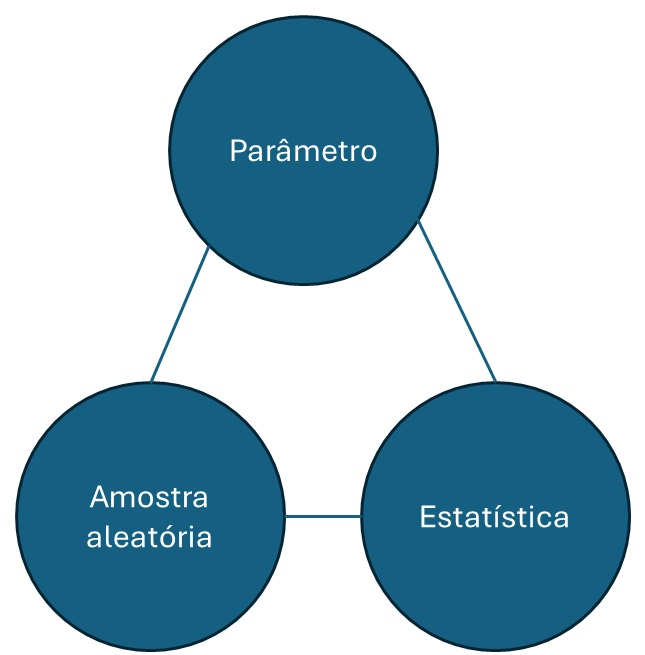
\includegraphics{fig_stat_geral.jpg}

}

\caption{A relação mais comum entre amostra, estatística e os parâmetros
populacionais}

\end{figure}%

Se a distribuição amostral da estatística não depende dos parâmetros,
dizemos que essa estatístca é ancilar. A figura abaixo representa a
relação entre a amostra aleatória, os parâmetros e esse tipo de
estatística.

\begin{figure}

{\centering 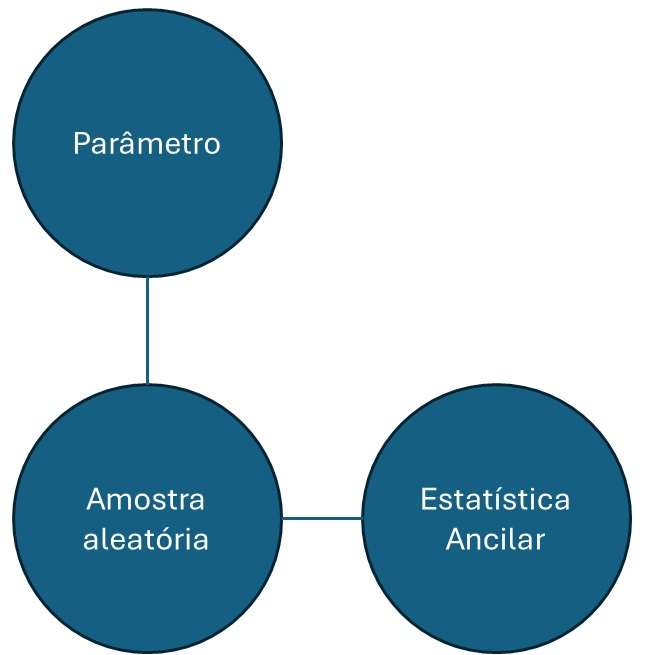
\includegraphics{fig_stat_ancilar.jpg}

}

\caption{Relação entre amostra, estatísticas ancilares e os parâmetros
populacionais}

\end{figure}%

\textbf{Exemplo} Seja \(X_1,\ldots,X_{n}\) uma amostra aleatória da
população Normal\((\mu,1)\). Sabemos que a distribuição amostral da
média amostral é
\[\bar{X}_n\sim\hbox{Normal}\left(\mu,\frac{1}{n}\right).\] Portanto,
\(\bar{X}_n\) carrega informação sobre \(\mu\). Considere agora a
estatística \[W=X_1-X_2.\] Note que \(W\) é uma combinação linear de
normais independentes, logo também possui distribuição normal. Como
\[E(W)=E(X_1)-E(X_2)=0\] e \[Var(W)=Var(X_1-X_2)=Var(X_1)+Var(X_2)=2,\]
temos que a distribuição amostral de \(W\) é Normal(0,2). Como essa
distribuição não depende de \(\mu\), temos que \(W\) não carrega
informação sobre o parâmetro e, portanto, é uma estatística ancilar.

\section{Estatísticas suficientes}\label{estatuxedsticas-suficientes}

Uma estatística é dita ser suficiente para \(\theta\) se, quando
observada, ela permite descrever a distribuição da amostra aleatória sem
o conhecimento de \(\theta\). Segue a definição formal.

\textbf{Definição.} Uma estatística \(T\) é dita ser suficiente para
\(\theta\) se a distribuição \(X_1,\ldots,X_n|T=t\) não depende de
\(\theta\).

A figura abaixo mostra a relação entre a amostra aleatória, os
parâmetros e a estatística suficiente. Observe que a depenência da
amostra em relação aos parâmetros se dá através da estatítica
suficiente. 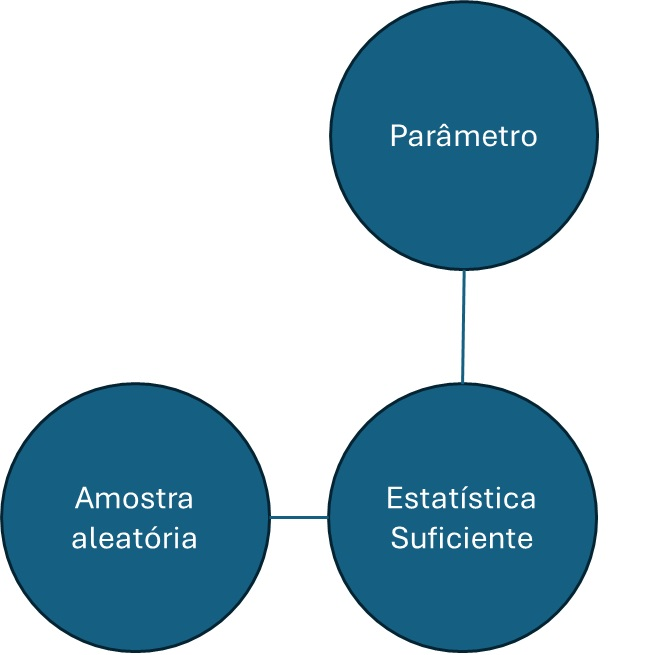
\includegraphics{fig_stat_suficiente.jpg}

Note que a própria amostra é uma estatística suficiente para \(\theta\).
De fato, considerando o caso discreto, pode-se notar que

\[P(\textbf{X}=\textbf{x}|\textbf{X}=\textbf{x},\boldsymbol{\theta})=\frac{P(\textbf{X}=\textbf{x},\textbf{X}=\textbf{x}|\boldsymbol{\theta})}{P(\textbf{X}=\textbf{x}|\boldsymbol{\theta})}=1,\]
que não depende de \(\theta\). O teorema a seguir é uma importante
ferramenta para encontrar estatísticas suficientes.

\textbf{Teorema do Critério da Fatoração de Neyman} Seja \(\textbf{X}\)
uma amostra aleatória cuja distribuição. Então, \(T\) é um estatística
suficiente para \(\theta\) se e somente se existem funções
\(h(\textbf{x})\) e \(g(T,\theta)\) tais que

\[\prod_{i=1}^nf(x_i|\theta)=h(\textbf{x})g(t,\theta)\] onde \(f\) é a
função de densidade ou a função de probabilidade da população.

\textbf{Exemplo} Seja \(X_1,\ldots,X_n\) uma amostra aleatória da
população Exponencial(\(\theta\)). Note que
\[\prod_{i=1}^n  f(x_i|\theta)=\prod_{i=1}^n \theta e^{-\theta x_i}=\underbrace{\theta^n}_{h(\textbf{x})}. \underbrace{e^{-\theta\sum_{i=1}^n x_i}}_{g(\sum_{i=1}^n x_i,\theta)},\]
logo, pelo Teorema do Critério da Fatoração, \(T=\sum_{i=1}^{n}X_i\) é
uma estatística suficiente para \(\theta\).

\textbf{Exemplo.} Seja \(X_1,\ldots,X_n\) uma amostra aleatória do
modelo \(X\sim\hbox{Poisson}(\lambda)\). Note que

\[P(\textbf{X}=\textbf{x}|\lambda)=\prod_{i=1}^n\frac{e^{-\lambda}\lambda^{x_i}}{x_i!}=\underbrace{\prod_{i=1}^n\frac{1}{x_i!}}_{h(\textbf{x})}.\underbrace{e^{-n\lambda}\lambda^{\sum_{i=1}^n x_i}}_{g(\sum_{i=1}^n x_i,\lambda)},\]
logo, pelo Teorema do Critério da Fatoração de Neyman,
\(T=\sum_{i=1}^n X_i\) é suficiente para \(\lambda\).

Quando há mais de uma estatística na fatoração, elas são denominadas
conjuntamente suficientes.

\textbf{Exemplo.} Seja \(X_1,\ldots,X_n\) uma amostra aleatóra da
população \(\hbox{Normal}(\mu,\sigma^2)\). Note que
\[f(\textbf{x}|\mu,\sigma^2)=\prod_{i=1}^n\left(\frac{1}{2\pi\sigma^2}\right)^{1/2} e^{-\frac{1}{2\sigma^2}(x_i-\mu)^2}=\left(\frac{1}{2\pi\sigma^2}\right)^{n/2} e^{-\frac{1}{2\sigma^2}\sum_{i=1}^n(x_i-\mu)^2}.\]
Como
\[\sum_{i=1}^n(x_i-\mu)^2=\sum_{i=1}^n x_i^2 +n\mu^2-2\mu\sum_{i=1}^n x_i,\]
teremos que
\[f(\textbf{x}|\mu,\sigma^2)=\underbrace{1}_{h(\textbf{x})}.\underbrace{\left(\frac{1}{2\pi\sigma^2}\right)^{n/2} e^{-\frac{1}{2\sigma^2}\left(\sum_{i=1}^n x_i^2 +n\mu^2-2\mu\sum_{i=1}^n x_i\right)}}_{g( \sum_{i=1}^n x_{i},\sum_{i=1}^n x_i^2,\mu,\sigma^2)}.\]
Portanto, pelo Teorema do Critério da Fatoração de Neyman,
\(\sum_{i=1}^nX_i\) e \(\sum_{i=1}^n X_i^2\) são conjuntamente
suficientes para \(\mu\) e \(\sigma^2\).

Você deve ter notado que todas as distribuições acima pertencem à
família exponencial. O teorema abaixo generaliza a busca de estatísticas
suficientes dentro dessa família.

\textbf{Teorema} Se \(X_1,\ldots,X_n\) é uma amostra aleatória de uma
população na família exponencial, então
\[T=\left\{\sum_{i=1}^n T_1(X_i),\ldots,\sum_{i=1}^n T_k(X_i)\right\}\]
é uma estatística suficiente para \(\theta\).

Vejamos alguns exemplos fora da família exponencial.

\textbf{Exemplo.} Seja \(X_1,\ldots,X_n\) uma amostra aleatória da
população Uniforme(0,\(\theta\)). Note que

\[\prod_{i=1}^n f(x_i|\theta)=\prod_{i=1}^n \frac{1}{\theta}I(x_i\leq \theta)=\frac{1}{\theta^n}\prod_{i=1}^{n}I(x_i\leq \theta).\]
O produtório acima é igual a 1 se e somente se todas as observações
forem menores ou iguais que \(\theta\). Para que isto ocorra, basta que
a maior das observações seja menor que \(\theta\). Denotando a
estatística máximo amostral por \(X_{(n)}\), teremos

\[\prod_{i=1}^nf(x_i|\theta)=\underbrace{1}_{h(\textbf{x})}.\underbrace{\frac{1}{\theta^n}I(x_{(n)}\leq\theta)}_{g(x_{(n)},\theta)},\]
logo, pelo Teorema do Critério da Fatoração de Neyman, teremos que
\(T=X_{(n)}\) é suficiente para \(\theta\).

\textbf{Importante} Sejam \(x_{(1)}\) e \(x_{(n)}\) as estatísticas
mínimo e máximo de uma amostra de tamanho \(n\). Então: -
\(\prod_{i=1}^n I(x_i\leq \theta)=I(x_{(n)}\leq \theta)\) -
\(\prod_{i=1}^n I(x_i\geq \theta)=I(x_{(1)}\geq \theta)\) -
\(\prod_{i=1}^n I(\alpha\leq x_i\leq \beta)=I(\alpha\leq x_{(1)})I(x_{(n)}\leq \beta)\)

\textbf{Exemplo.} Seja \(X_1,\ldots,X_n\) uma amostra aleatória da
população cuja função densidade é dada por

\[f(x|\mu)=e^{-(x-\mu)}I(x\geq \mu).\] Esse modelo é conhecido como
exponencial deslocada. Contudo, como os valores de \(x\) dependem de
\(\mu\), esta distribuição não está na família exponencial. Observe que
\[\prod_{i=1}^n f(x_i|\mu)=\prod_{i=1}^n e^{-(x_i-\mu)}I(x_i\geq \mu)=e^{-\sum_{i=1}^n x_i}e^{n\mu}\prod_{i=1}^{n}I(x_i\geq \mu).\]
O produtório acima é igual a 1 se e somente se todas as observações
forem maiores ou iguais que \(\mu\). Para que isto ocorra, basta que
\(x_{(1)}\) seja maior que \(\mu\). Então, teremos que

\[\prod_{i=1}^nf(x_i|\theta)=\underbrace{e^{-\sum_{i=1}^n x_i}}_{h(\textbf{x})}.\underbrace{e^{n\mu}I(x_{(1)}\geq \mu)}_{g(x_{(1)},\mu)},\]
logo, pelo Teorema do Critério da Fatoração de Neyman, teremos que
\(T=X_{(1)}\) é suficiente para \(\mu\).

\textbf{Exemplo.} Seja \(X_1,\ldots,X_n\) uma amostra aleatória da
população Uniforme(\(\alpha,\beta\)), cuja densidade é dada por

\[f(x|\alpha,\beta)=\frac{1}{\beta-\alpha}I(\alpha\leq x\leq \beta).\]
Sem perda de generalidade, podemos reescrever
\[I(\alpha\leq x\leq \beta)=I(\alpha\leq x)I(x\leq\beta),\] logo,

\[\begin{align}\prod_{i=1}^n f(x_i|\alpha,\beta)&=\prod_{i=1}^n \frac{1}{\beta-\alpha}I(\alpha\leq x_i)I(x_i\leq\beta)\\&=\underbrace{1}_{h(\textbf{x})}.\underbrace{\frac{1}{(\beta-\alpha)^n}I(\alpha\leq x_{(1)})I(x_{(n)}\leq\beta)}_{g(x_{(1)},x_{(n)},\alpha,\beta
)}.\end{align}\] logo, pelo Teorema do Critério da Fatoração de Neyman,
teremos que \(X_{(1)}\) e \(X_{(n)}\) são conjuntamente suficientes para
\(\alpha\) e \(\beta\).

\bookmarksetup{startatroot}

\chapter*{References}\label{references}
\addcontentsline{toc}{chapter}{References}

\markboth{References}{References}

\phantomsection\label{refs}
\begin{CSLReferences}{0}{1}
\end{CSLReferences}



\end{document}
